\documentclass[10pt,journal]{IEEEtran}
%\IEEEoverridecommandlockouts

\usepackage[spanish,es-tabla]{babel} % Idioma español con tablas
\usepackage[spanish]{babel}
\usepackage[table,xcdraw]{xcolor} % Para pintar tablas
\usepackage{url} % Para colocar URL
\usepackage{amsmath,amssymb,amsfonts}
\usepackage{graphicx}
\usepackage{textcomp}
\usepackage{xcolor}
\usepackage{float} % Para var H, figure

\usepackage[square,numbers]{natbib}
\bibliographystyle{abbrvnat}

\renewcommand{\baselinestretch}{1.5}     %interlineado

\title{Instrumentos de Recolección de Datos en Informática o Ciencias de la Computación}

\author{
\IEEEauthorblockN{{\Large Angely Mendez Cruz}} \\
\vspace{2mm}
\IEEEauthorblockA{\textit{Metodología de la Investigación Científica} \\
\textit{Escuela de Informática} \\
\textit{Facultad de Ciencias Físicas y Matemáticas} \\
\textit{Universidad Nacional de Trujillo, \\ Perú }
\\ \vspace{1mm}
t052701020@unitru.edu.pe}}

\begin{document}
\renewcommand{\IEEEkeywordsname}{{\bfseries Palabras claves:}} % Colocar Keywords en Spanish

\maketitle

    \begin{abstract}
    En este trabajo de investigación se brinda información respecto a dos temas en específico, los cuales son: Sistemas Criptográficos y Minería de Datos, en las que se evidencia dos aplicaciones de la informática en la realidad; exponiendo una breve descripción de lo realizado y sus resultados, además enfatizando en los instrumentos de recolección de datos de cada una de ellas donde se ha considerado la observación y otros recursos que le permitieron a los investigadores acercarse al objeto de estudio, también fueron empleados los conocimientos sobre ciencias de la computación, la tecnología existente y la propuesta e incluso ejecución de nuevas tecnologías propias, algoritmos eficientes e investigaciones externas.
    \end{abstract}
    
    \begin{IEEEkeywords}
    Instrumentos, recolección de datos, informática, ciencias de la computación.
    \end{IEEEkeywords}
    
    \section{\textbf{Introducción}}
    
    En la actualidad y ante el planteamiento de resolver problemáticas, los instrumentos de recolección de datos son en principio cualquier recurso del cual pueda valerse el investigador para acercarse a los fenómenos y extraer de ellos información. Para muchos pareciera que la elección de los instrumentos a emplear es fácil, y lo es, siempre y cuando el investigador tenga experiencia en el campo investigativo y amplios conocimientos en su área disciplinaria.
    
    El instrumento sintetiza en si toda la labor previa de la investigación, resume los aportes del marco teórico al seleccionar datos que corresponden a los indicadores y, por lo tanto a las variables o conceptos utilizados. Dentro de la informática o Ciencias de la Computación existen diversos temas en los que se emplean ellos, antes se debe tener conocimiento respecto a la metodología dentro de la investigación, teniendo en cuenta el análisis de la realidad.

    Algunas de las funciones de los instrumentos de recolección de datos son dirigir, recolectar, conservar, reelaborar y transmitir los datos, es decir son los medios, a través de los cuales se hace posible la obtención y archivo de la información, en el presente artículo se expone dos temas dentro de la informática, sus aplicaciones y la utilización de sus instrumentos.  

    \section{\textbf{Instrumentos de Recolección de Datos en Informática o Ciencias de la Computación}}
    \subsection{\underline{\textbf{Sistemas Criptográficos}}}
    Según Saéz Hurtado \citep{cripto}, la criptografía es un método de protección de la información y las comunicaciones mediante el uso de códigos, de modo que solo aquellos a quienes está destinada la información puedan leerla y procesarla. El origen del término, deriva del prefijo \textbf{\textit{cripta}} significa \textit{oculto} o \textit{bóveda} y el sufijo \textbf{\textit{-grafía}} significa \textit{escritura}.

    En el campo de la informática \citep{marrero}, los sistemas criptográficos se refieren al conjunto de procesos y/o técnicas de comunicación e información seguras derivadas de conceptos matemáticos y cálculos basados en reglas llamados \textbf{algoritmos}, para transformar los mensajes en formas difíciles de descifrar.
    
    \begin{figure}[H]
      \begin{center}
        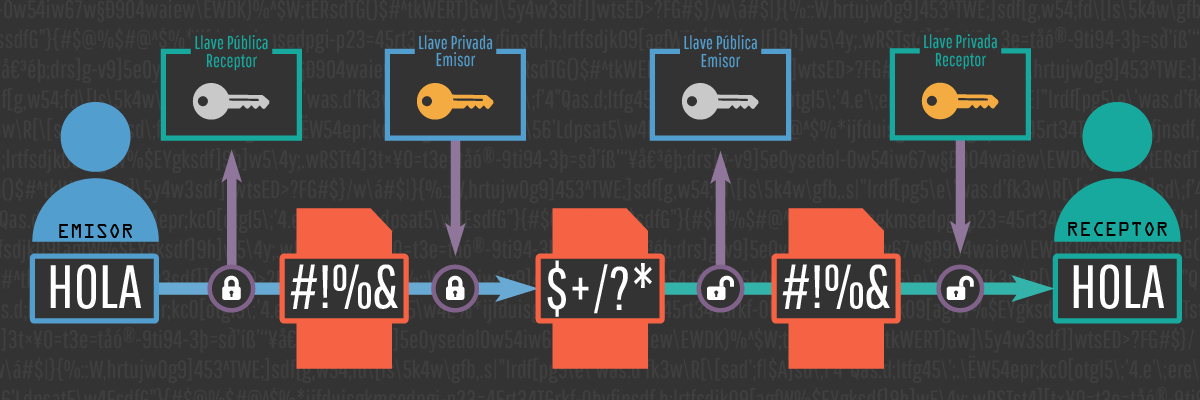
\includegraphics[width=7.7cm, height=3.5cm]{figuras/cripto.png}
        \caption{Sistema Criptográfico - Tomado de la Dirección Nacional del Registro de Dominios de Internet (NIC Argentina).}
        \label{cripto} 
        \end{center}
    \end{figure}
    
     Estos algoritmos deterministas se utilizan para la generación de claves criptográficas, firma digital, verificación para proteger la privacidad de los datos, navegación web en Internet y comunicaciones confidenciales como transacciones con tarjetas de crédito y correo electrónico, tal como se muestra en la Figura ~\ref{cripto}.
    
    A continuación, una investigación respecto a la aplicación de los sistemas criptográficos:
    \begin{itemize}
        \item Históricamente, la autentificación de paquetes se ha manejado a través de firmas digitales basadas en certificados, usualmente emitidos por una entidad neutral a la comunicación y de confianza de todas las partes. Sin embargo, esta solución no siempre es posible de implementar, debido a factores como los costos, el tiempo limitado de vigencia de los certificados, la necesidad de depositar la confianza en un tercero, y por último el poder, usualmente limitado, de procesamiento de las máquinas.
            
    \begin{figure}[H]
      \begin{center}
        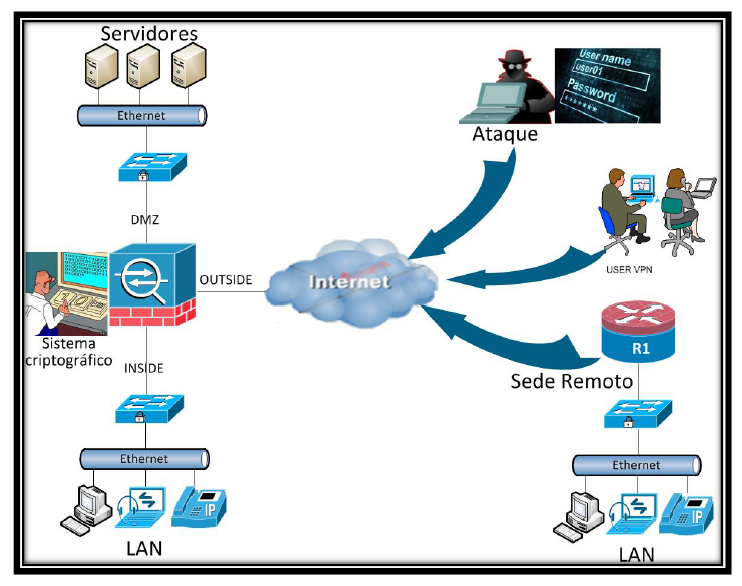
\includegraphics[width=7cm, height=4cm]{figuras/criptoinv.PNG}
        \caption{Diagrama Contextual del Sistema Criptográfico.}
        \label{criptoinv} 
        \end{center}
    \end{figure}
        
        Por lo que la tesis de título \textit{“Implementación de un sistema criptográfico a través de algoritmos avanzados de encriptación para mejorar la seguridad perimetral de una red informática"}, \citep{guevara} tiene como objetivo desarrollar una alternativa de sistema de seguridad para la red informática, tal como se muestra en la Figura ~\ref{criptoinv}. El sistema utiliza algoritmos avanzados para la encriptación y desencriptación de los paquetes de información enviados en la entidad de estudio para la protección de datos privados del usuario. 
        
        El diseño de la investigación fue \textbf{no experimental}, debido que no se pretendió variar intencionalmente variables independientes por lo que se observaron los fenómenos tal y como se dan en su contexto. Esto se debe a las limitaciones sobre el costo de implantación y el tiempo prolongado de obtención de resultados.
        
    \begin{figure}[H]
      \begin{center}
        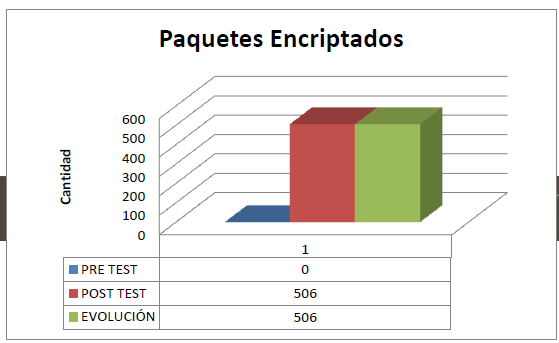
\includegraphics[width=7cm, height=4cm]{figuras/criptoinv3.PNG}
        \caption{Muestra de la Investigación.}
        \label{criptoinv3} 
        \end{center}
    \end{figure}
        
        El trabajo tuvo como \textbf{población}, a la cantidad de data enviada y recibida en la red perimetral de la institución “ABACO”, es decir todo el tráfico IP permitido entre la red origen y destino, ver Figura ~\ref{criptoinv3}. Debido a que se tiene acceso a la red perimetral del Instituto Superior Tecnológico Privado “ABACO”, la \textbf{muestra} trabaja con toda la población.
        
        Las \textbf{técnicas e instrumentos de recolección de datos}, utilizadas en la presente investigación, son las detalladas a continuación:
        \begin{enumerate}
        \item \textit{Guía de observación de la bitácora sobre datos del sistema criptográfico}: Se observó los datos almacenados en la bitácora del sistema criptográfico para la comparación de resultados antes y después de hacerle las pruebas al sistema.
        \item \textit{Guía de plan de pruebas del sistema criptográfico}: Se observó los procesos de pruebas que se le hacen al sistema para ver si se logró cumplir con el objetivo planteado en la presente investigación, el cual está dado por la mejora de la seguridad perimetral de la red informática de la institución, ver Figura ~\ref{criptoinv2}.
        \end{enumerate}

    \begin{figure}[H]
      \begin{center}
        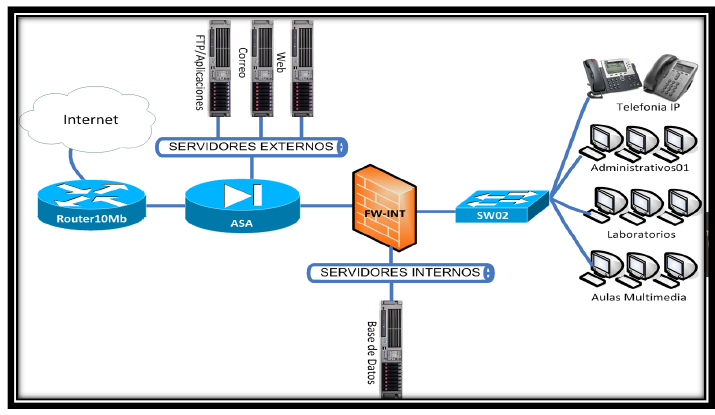
\includegraphics[width=7cm, height=4cm]{figuras/criptoinv2.PNG}
        \caption{Diagrama Lógico Actual del Sistema.}
        \label{criptoinv2} 
        \end{center}
    \end{figure}     
    
        El desarrollo de este trabajo consistió en un estudio de las componentes a usar, tanto de hardware como de software, incluyendo los conceptos básicos necesarios para su diseño y operación, así como los estándares y metodologías que siguen. Este proceso se llevó a cabo mediante el diseño de la estructura y la topología la cual fue implementada en un prototipo, obsérvese en la Figura ~\ref{criptoinv4}. y finalmente se documentó.
        
      \begin{figure}[H]
      \begin{center}
        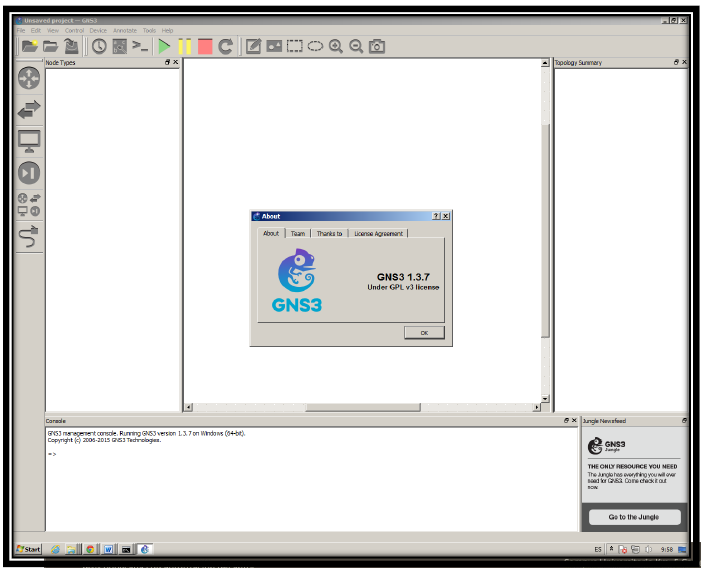
\includegraphics[width=7cm, height=4cm]{figuras/criptoinv4.PNG}
        \caption{Diagrama Lógico Actual del Sistema.}
        \label{criptoinv4} 
        \end{center}
    \end{figure}
    \end{itemize}
    
    \subsection{\underline{\textbf{Minería de Datos}}}
    Según lo define Minewiskan \citep{Conceptomine}, la minería de datos es el proceso de detectar la información procesable de los conjuntos grandes de datos, obsérvese en la Figura ~\ref{miner45}. Utiliza el análisis matemático para deducir los patrones y tendencias que existen en los datos. Normalmente, estos patrones no se pueden detectar mediante la exploración tradicional de los datos porque las relaciones son demasiado complejas o porque hay demasiado datos.
    
    \begin{figure}[H]
      \begin{center}
        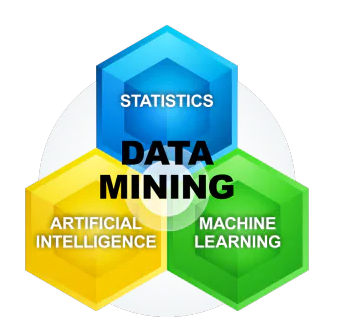
\includegraphics[width=5cm, height=4cm]{figuras/miner45.PNG}
        \caption{Campos de la Minería de Datos - Tomado de Soluciones Analíticas (SAS Perú).}
        \label{miner45} 
        \end{center}
    \end{figure}  
    
    Un algoritmo en minería de datos (o aprendizaje automático) es un conjunto de heurísticas y cálculos que permiten crear un modelo a partir de datos \citep{mineria2}. Para crear un modelo, el algoritmo analiza primero los datos proporcionados, en busca de tipos específicos de patrones o tendencias. El algoritmo usa los resultados de este análisis en un gran número de iteraciones para determinar los parámetros óptimos para crear el modelo de minería de datos.
    
    A continuación, una investigación respecto a la aplicación de la minería de datos:
    \begin{itemize}
        \item  En la actualidad, la administración de la información es el eje fundamental en toda organización, especialmente para apoyar los procesos del negocio que se basan en recursos de información, tomando fuerza la tarea de mejorar el acceso a los datos. 
        
        De acuerdo con la idea del párrafo anterior, la tesis titulada, \textit{“Minería de datos para mejorar la toma decisiones en el área de gestión al cliente de telefónica del Perú zonal Tarapoto”}, \citep{uriarte} tiene como objetivo general, determinar el efecto del uso de minería de datos en la toma de decisiones en el área de gestión al cliente de telefónica del Perú zonal Tarapoto. 
        
        Para cumplir con tal objetivo se tuvo que analizar los procesos de toma de decisiones en el área de gestión al cliente encontrando ciertas falencias; teniendo en claro el análisis se pasó a diseñar e implementar el sistema con herramientas de minería de datos llevando a medir los resultados en el proceso de toma de decisiones con el uso del aplicativo con minería de datos.
        
        \begin{figure}[H]
      \begin{center}
        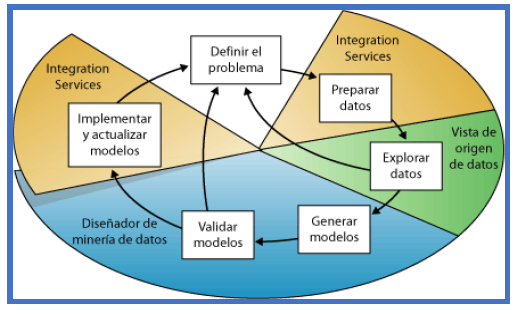
\includegraphics[width=7cm, height=5cm]{figuras/mininv.PNG}
        \caption{Pasos ejecutados en la investigación.}
        \label{mininv} 
        \end{center}
    \end{figure}  
        
         Para el desarrollo de la investigación se tomó como base el entorno actual de la minería de datos ya que se presentó un análisis de su importancia, origen e implementación, pasando por la descripción de las metodologías existentes para desarrollar un proyecto, como se muestra en la Figura ~\ref{mininv}. A su vez, hace de su manejo en los procesos empresariales relacionados con la estrategia de Customer Relationship Management (crm) para la toma decisiones empresariales y el fraccionamiento del cliente.
         
         \begin{figure}[H]
      \begin{center}
        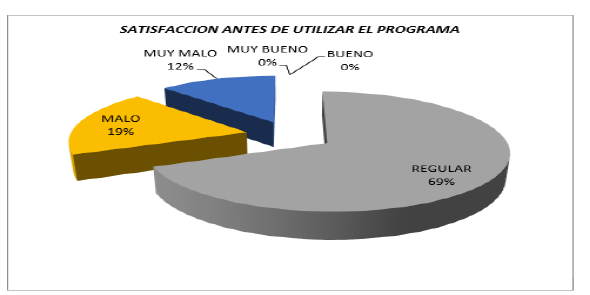
\includegraphics[width=7cm, height=5cm]{figuras/mininv4.PNG}
        \caption{Satisfacción antes de Usar el Programa.}
        \label{mininv4} 
        \end{center}
    \end{figure} 
         
        La \textbf{población y muestra} del trabajo fue el correspondiente a la oficina de gestión al cliente de la zonal Tarapoto, de telefónica del Perú ubicada en la jurisdicción de la Provincia y Departamento de San Martín y específicamente en el Distrito de Tarapoto, como se muestra la satisfacción en la Figura ~\ref{mininv4}.
         
        Mientras que los \textbf{instrumentos de recolección de datos} fueron los que se detallan a continuación:
        \begin{enumerate}
        \item \textit{Cartilla de observación}: Debido a que se aplicó en el proceso de toma de decisiones en el área de gestión al cliente sistema de control.
        \item \textit{Sistema de Minería de datos}: Establecido para los procesos de toma de decisiones en el área de gestión al cliente.
        \item \textit{Fichas bibliográficas y Subrayado}: Ejecutado en la bibliografía necesaria para desarrollar el marco teórico y la información complementaria.
        \end{enumerate} 
        
        Además, los \textbf{instrumentos de procesamiento de datos} para mayor precisión, fueron obtenidos, ordenados y procesados con la ayuda del software estadístico SPSS. Donde se elaborarán cuadros descriptivos para presentar los datos obtenidos por cada variable e indicador después de la experimentación.
        
        \begin{figure}[H]
      \begin{center}
        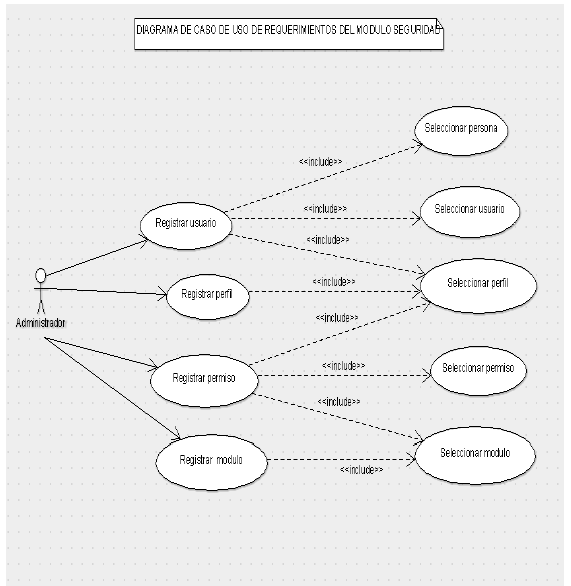
\includegraphics[width=8cm, height=5cm]{figuras/mininv2.PNG}
        \caption{Resultados obtenido del lenguaje programación PHP.}
        \label{mininv2} 
        \end{center}
    \end{figure} 
        
        Para la culminación de este proyecto se hizo el levantamiento de información se utilizaron técnicas de observación; para el análisis y diseño se utilizó el UML, ver Figura Figura ~\ref{mininv2}, que es un lenguaje de modelado visual y se utilizó la metodología RUP (proceso racional unificado). También se generó un Chart de visualización sobre el porcentaje de avance de objetivos según un producto, como se muestra en la Figura ~\ref{mininv3}.
        
            \begin{figure}[H]
      \begin{center}
        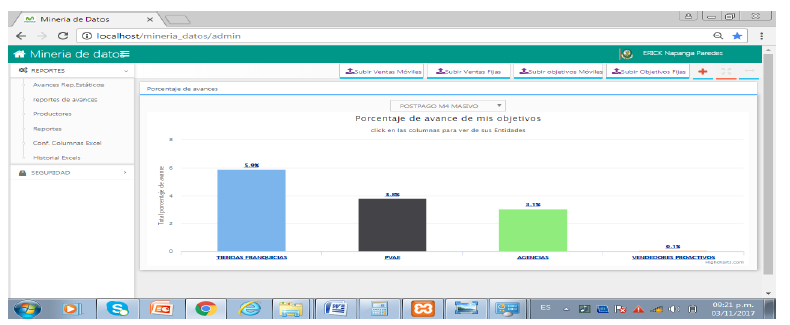
\includegraphics[width=8cm, height=5cm]{figuras/mininv3.PNG}
        \caption{Resultados obtenido del lenguaje programación PHP.}
        \label{mininv3} 
        \end{center}
    \end{figure} 
    \end{itemize}

    \section{\textbf{Conclusiones}}
    Para concluir, las dos investigaciones presentadas en este trabajo,  que son aplicaciones que se establecen bajo dos temas tales como Sistemas Criptográficos y Minería de Datos, demuestran que sus aportes en el campo de la informática son diversas y muy útiles en la sociedad. Así como los instrumentos de recolección de datos que utilizaron para cumplir sus objetivos y desarrollar de manera correcta los mismos, fueron los adecuados desde el punto de vista de las ciencias de la computación porque se aplicaron en un momento en particular, con la finalidad de buscar y obtener información que les fue útil para los objetos de estudio. Finalmente, las investigaciones en la informática expuestas en este trabajo de recopilación, sirven como antecedentes y base a futuros investigadores a nivel nacional e internacional, que pueden ser usados tanto en el área comercial o académico.
\medskip
\bibliography{Referencia}

\end{document}
